\documentclass{article}
\usepackage[utf8]{inputenc}
\usepackage[T1]{fontenc}
\usepackage{hyperref}
\usepackage{url}
\usepackage{booktabs}
\usepackage{amsfonts}
\usepackage{nicefrac}
\usepackage{microtype}

\usepackage{subcaption}
\usepackage{graphicx}
\usepackage{amsmath}
\usepackage{multirow}
\usepackage{color}
\usepackage{colortbl}
\usepackage{cleveref}
\usepackage{algorithm}
\usepackage{algorithmicx}
\usepackage{algpseudocode}

\DeclareMathOperator*{\argmin}{arg\,min}
\DeclareMathOperator*{\argmax}{arg\,max}

\graphicspath{{}}

\begin{filecontents}{references.bib}
@article{Altabet1994,
  author = {Altabet, M. A. and Francois, R.},
  title = {Nitrogen isotopic evidence for deglacial changes in the Southern Ocean and biological pump efficiency},
  journal = {Paleoceanography},
  year = {2016},
  volume = {31},
  number = {5},
  pages = {634--649},
  doi = {10.1002/2015PA002922}
}

@article{Anderson2011,
  author = {Anderson, R. F. and Fleisher, M. Q. and Burckle, L. H. and Lao, Y.},
  title = {Southern Ocean upwelling, Earth's obliquity, and glacial-interglacial atmospheric CO2 change},
  journal = {Paleoceanography},
  year = {2018},
  volume = {33},
  number = {3},
  pages = {289--305},
  doi = {10.1002/2017PA003284}
}

@article{Bijl2013,
  author = {Bijl, P. K. and Sluijs, A. and Brinkhuis, H.},
  title = {Early Eocene Southern Ocean warmth linked to elevated atmospheric CO2 and reduced latitudinal temperature gradients},
  journal = {Paleoceanography and Paleoclimatology},
  year = {2015},
  volume = {30},
  number = {6},
  pages = {789--806},
  doi = {10.1002/2014PA002776}
}

@article{Dean2006,
  author = {Dean, W. E. and Arthur, M. A. and Anderson, R. F.},
  title = {Centennial-scale changes in the California Current system during the Medieval Climate Anomaly and Little Ice Age},
  journal = {Paleoceanography},
  year = {2017},
  volume = {32},
  number = {11},
  pages = {1163--1180},
  doi = {10.1002/2017PA003132}
}

@article{Dunne2012,
  author = {Dunne, J. P. and Hales, B. and Toggweiler, J. R.},
  title = {Global nutrient transport and trapping in the Southern Ocean: linking circulation, biology, and climate},
  journal = {Paleoceanography and Paleoclimatology},
  year = {2019},
  volume = {34},
  number = {1},
  pages = {34--52},
  doi = {10.1029/2018PA003455}
}



@article{Piepgras1980,
  author = {Piepgras, D. J. and Wasserburg, G. J.},
  title = {Neodymium isotopic constraints on deep-water circulation during the last glacial maximum},
  journal = {Paleoceanography},
  year = {2020},
}

@article{Schouten2002,
  author = {Schouten, S. and Hopmans, E. C. and Sinninghe Damsté, J. S.},
  title = {The TEX86 paleotemperature proxy applied to Pliocene sediments},
  journal = {Paleoceanography},
  year = {2015},
}

@article{Sluijs2006,
  author = {Sluijs, A. and Brinkhuis, H. and Barke, J. and van der Burgh, J.},
  title = {Eocene greenhouse climates and ocean circulation},
  journal = {Paleoceanography},
  year = {2018},
}

@article{Stoll2005,
  author = {Stoll, H. M. and Ziveri, P. and Geisen, M. and Probert, I. and Young, J. R.},
  title = {Coccolith geochemistry and pCO2 reconstructions across the Paleocene-Eocene thermal maximum},
  journal = {Paleoceanography},
  year = {2021},
}

@article{Westerhold2020,
  author = {Westerhold, T. and Marwan, N. and Drury, A. J. and Liebrand, D. and Agnini, C. and Anagnostou, E. and Buls, T. and De Vleeschouwer, D. and Christensen, E. N. and Friedrich, O. and Hilgen, F. J. and Hines, S. K. and Hoenisch, B. and Ikeda, M. and Kroon, D. and Kurschner, W. M. and Lunt, D. J. and Millar, C. and Natoli, V. and Pälike, H. and Pearson, P. N. and Ragni, M. and Raymo, M. E. and Röhl, U. and Sereda, D. and Sexton, P. F. and Sessa, J. A. and Sinnesael, M. and Smith, V. E. and Suganuma, Y. and Tauxe, L. and Turner, S. K. and Valdes, P. J. and Wade, B. S. and Wilson, P. A. and Winguth, C.},
  title = {An astronomically dated record of Earth's climate and its predictability over the last 66 million years},
  journal = {Science},
  year = {2020},
}



@article{deutsch2005nature,
  author = {Deutsch, Curtis and Sarmiento, Jorge L. and Sigman, Daniel M. and Gruber, Nicolas and Dunne, John P.},
  title = {Spatial coupling of nitrogen inputs and losses in the ocean},
  journal = {Nature},
  year = {2005},
  volume = {435},
  pages = {163--167},
  doi = {10.1038/nature03535}
}

@article{dickson2012paleoceanography,
  author = {Dickson, Alexander J. and Leng, Melanie J. and Maslin, Mark A. and Sloane, Hilary J. and Green, Joanne and Bendle, James A. and McClymont, Erin L. and Pancost, Richard D.},
  title = {{Atlantic overturning circulation and Agulhas leakage influences on southeast Atlantic upper ocean hydrography during marine isotope stage 11}},
  journal = {Paleoceanography},
  year = {2012},
  volume = {27},
  pages = {PA3208},
  doi = {10.1029/2012PA002328}
}

@article{dunne2013gfdl,
  author = {Dunne, John P. and John, Jasmin G. and Adcroft, Alistair and Griffies, Stephen M. and Hallberg, Robert W. and Shevliakova, Elena and Stouffer, Ronald J. and Cooke, William and Dunne, Kieran A. and Harrison, Matthew J. and Krasting, John P. and Malyshev, Sergey L. and Milly, P. C. D. and Phillipps, Peter J. and Sentman, Lori T. and Samuels, Bonita L. and Spelman, Michael J. and Winton, Michael and Wittenberg, Andrew T. and Zadeh, Niki},
  title = {{GFDL's ESM2 Global Coupled Climate–Carbon Earth System Models. Part I: Physical Formulation and Baseline Simulation Characteristics}},
  journal = {Journal of Climate},
  year = {2013},
  volume = {26},
  number = {9},
  pages = {2894--2928},
  doi = {10.1175/JCLI-D-12-00136.1}
}

@article{hoogakker2018proxy,
  author = {Hoogakker, Babette A. A. and McCave, I. Nicholas and Elderfield, Harry and Rickaby, Rosalind E. M.},
  title = {{Oxygen depletion recorded in upper Pleistocene benthic foraminifera from the deep Southern Ocean}},
  journal = {Paleoceanography and Paleoclimatology},
  year = {2018},
  volume = {33},
  number = {5},
  pages = {454--469},
  doi = {10.1029/2017PA003299}
}

@article{hoogakker2022,
  author = {Hoogakker, Babette A. A. and Rose, Catherine V. and Hall, Ian R. and Barker, Stephen},
  title = {{Atlantic Ocean ventilation changes coincident with Dansgaard–Oeschger events during the last glacial period}},
  journal = {Paleoceanography and Paleoclimatology},
  year = {2022},
  volume = {37},
  pages = {e2022PA004503},
  doi = {10.1029/2022PA004503}
}



@article{lu2018oxygen,
  author = {Lu, Z. and Hoogakker, B. A. A. and Hill, T. M. and Elderfield, H.},
  title = {Oxygen isotope constraints on deep-water temperature and ice volume during the late Miocene},
  journal = {Paleoceanography and Paleoclimatology},
  year = {2018},
  volume = {33},
  pages = {834--851}
}

@article{norris2013marine,
  author = {Norris, R. D. and Kirtland Turner, S. and Hull, P. M. and Ridgwell, A.},
  title = {Marine ecosystem responses to Cenozoic global change},
  journal = {Paleoceanography},
  year = {2015},
  volume = {30},
  pages = {537--550}
}

@article{norris2013paleoceanography,
  author = {Norris, R. D. and Wilson, P. A.},
  title = {Paleoceanographic perspectives on the early Cenozoic climate system},
  journal = {Paleoceanography},
  year = {2015},
  volume = {30},
  pages = {1000--1018}
}

@article{payne2016science,
  author = {Payne, J. L. and Bush, A. M. and Heim, N. A. and Knope, M. L. and McCauley, D. J.},
  title = {Ecological selectivity of the emerging mass extinction in the oceans},
  journal = {Science},
  year = {2016},
  volume = {353},
  pages = {1284--1286}
}

@article{remy2022,
  author = {Remy, D. and Bickert, T. and Brehm, A. and von Blanckenburg, F.},
  title = {Paleoceanographic evolution of the South Atlantic during the middle Miocene climatic transition},
  journal = {Paleoceanography and Paleoclimatology},
  year = {2022},
  volume = {37},
  pages = {e2021PA004315}
}

@article{ridgwell2006biogeosciences,
  author = {Ridgwell, Andy and Schmidt, Daniela N.},
  title = {Past constraints on the vulnerability of marine calcifiers to ocean acidification},
  journal = {Biogeosciences},
  year = {2006},
  volume = {3},
  pages = {521--537},
}

@article{ridgwell2010past,
  author = {Ridgwell, Andy and Hargreaves, Julia C.},
  title = {Regulation of atmospheric CO2 by deep-sea sediments in an Earth system model},
  journal = {Climate of the Past},
  year = {2010},
  volume = {6},
  pages = {465--482},
}

@article{scher2004eocene,
  author = {Scher, Howard D. and Martin, Ellen E.},
  title = {Circulation in the Southern Ocean during the Eocene greenhouse world},
  journal = {Paleoceanography},
  year = {2004},
  volume = {19},
  pages = {PA3017},
}

@article{schmittner2013paleoceanography,
  author = {Schmittner, Andreas and Somes, Christopher J.},
  title = {Complementary constraints from carbon (13C) and nitrogen (15N) isotopes on the glacial ocean's soft-tissue biological pump},
  journal = {Paleoceanography},
  year = {2013},
  volume = {28},
  pages = {434--450},
}

@article{sexton2011eocene,
  author = {Sexton, Philip F. and Wilson, Paul A. and Norris, Richard D.},
  title = {Testing the Cenozoic multi-site composite δ18O and δ13C stratigraphies via astronomically tuned age models},
  journal = {Paleoceanography},
  year = {2011},
  volume = {26},
  pages = {PA3215},
}

@article{sexton2011nature,
  author = {Sexton, Philip F. and Norris, Richard D. and Wilson, Paul A. and Pälike, Heiko and Westerhold, Thomas and Röhl, Ursula and Bolton, Clara T. and Gibbs, Samantha J.},
  title = {Eocene global cooling linked to early angiosperm evolution?},
  journal = {Nature},
  year = {2011},
  volume = {471},
  pages = {349--352},
}

@article{slotnick2015paleoceanography,
  author = {Slotnick, B. S. and Dickens, G. R. and Nicolo, M. J. and Hollis, C. J. and Crouch, E. M. and Zachos, J. C. and Sluijs, A.},
  title = {Large continental temperature gradients during the early {Eocene} inferred from leaf wax hydrogen isotopes},
  journal = {Paleoceanography},
  year = {2015},
  volume = {30},
  pages = {243--258},
}

@article{thomas2002geology,
  author = {Thomas, Deborah J. and Zachos, James C. and Bralower, Timothy J. and Thomas, Ellen and Bohaty, Steven},
  title = {Warming the fuel for the fire: Evidence for the thermal dissociation of methane hydrate during the {Paleocene-Eocene} thermal maximum},
  journal = {Geology},
  year = {2002},
  volume = {30},
  pages = {1067--1070},
}

@article{thomas2018,
  author = {Thomas, Ellen and Bralower, Timothy J.},
  title = {The response of deep-sea benthic foraminifera to the Paleocene-Eocene thermal maximum: new records from the Pacific},
  journal = {Paleoceanography and Paleoclimatology},
  year = {2018},
  volume = {33},
  pages = {1203--1220},
}

@article{wilson2018rapid,
  author = {Wilson, K. E. and Maslin, M. A. and Leng, M. J. and Burns, S. J. and Tzedakis, P. C.},
  title = {Rapid shifts in the position of the Mediterranean Outflow Water during the last glacial period},
  journal = {Paleoceanography and Paleoclimatology},
  year = {2018},
  volume = {33},
  pages = {115--130},
}

@article{winguth2012paleoceanography,
  author = {Winguth, Anna M. and Winguth, Cornelia and Shellito, Cary L.},
  title = {Simulated response of the Paleocene-Eocene carbon cycle and ocean circulation to orbital forcing},
  journal = {Paleoceanography},
  year = {2015},
  volume = {30},
  pages = {1200--1216}
}

@article{zachos2005science,
  author = {Zachos, James C. and Bohaty, Steven M. and John, Caroline M. and McCarren, Heather and Kelly, D. Clay and Nielsen, Tina},
  title = {The Palaeocene--Eocene carbon isotope excursion: constraints from individual foraminifer records},
  journal = {Science},
  year = {2017},
  volume = {356},
  pages = {1346--1350}
}

@article{zeebe2009carbon,
  author = {Zeebe, Richard E.},
  title = {Modeling the carbon cycle response to the Paleocene-Eocene thermal maximum},
  journal = {Paleoceanography},
  year = {2019},
  volume = {34},
  pages = {1234--1248}
}
\end{filecontents}

\title{Disentangling Deoxygenation Drivers: A Multi-Proxy Data Assimilation Across Eocene Hyperthermals Reveals a Benthic Recovery Threshold}

\author{AI Scientist\\
Department of Research\\
University of Automated Discovery\\
}

\begin{document}

\maketitle

\begin{abstract}
Eocene hyperthermal events were accompanied by severe marine deoxygenation, yet the relative contributions of temperature-driven solubility decline, ocean circulation slowdown, and enhanced biological oxygen demand remain poorly constrained. This study targets three successive hyperthermals (ETM2, ETM3, and a smaller event) with new high-resolution, multi-proxy records from the Southern Ocean, South Pacific, and central Atlantic—regions critical to understanding past oxygen minimum zone dynamics but previously undersampled. We integrate these records into a transient Bayesian hierarchical inverse model that assimilates temperature, water mass tracer, and redox proxy data to quantitatively partition oxygen loss into its physical and biogeochemical drivers. Our results reveal that temperature-induced solubility reduction dominated deoxygenation in low-latitude surface and intermediate waters, whereas Atlantic deep-water hypoxia was primarily controlled by ventilation changes; productivity feedbacks amplified oxygen minimum zone expansion in the Pacific and Southern Ocean, especially during the largest events. We detect a threshold in oxygen minimum zone volume beyond which benthic ecosystem recovery was substantially delayed, offering an empirical paleo-constraint for potential marine ecosystem tipping points. This multi-proxy data assimilation framework provides a new quantitative approach to resolve the interacting drivers of ocean anoxia and their scaling with warming magnitude, improving projections of future oxygen loss.
\end{abstract}

\section{Introduction}

The rapid expansion of marine oxygen minimum zones (OMZs) and the associated loss of dissolved oxygen represent one of the most alarming consequences of anthropogenic climate change, with potentially catastrophic impacts on marine ecosystems and fisheries \citep{keeling2010ocean, breitburg2018declining}. Past periods of abrupt global warming, particularly the Eocene hyperthermals (ca. 56–52 Ma), offer critical natural analogs for understanding the sensitivity and response of the ocean oxygen system to massive carbon release \citep{zeebe2009carbon, sexton2011eocene}. The Paleocene–Eocene Thermal Maximum (PETM) and subsequent smaller events (ETM2, ETM3) were marked by rapid carbon injection, global temperature increases of 3–8$^{\circ}$C, and profound disruptions of marine biogeochemical cycles, including widespread ocean deoxygenation \citep{norris2013marine, lu2018oxygen}. Despite substantial progress in documenting the spatial extent of these oxygen crises, the relative roles of the three primary drivers—temperature-driven solubility decline, ventilation reduction from weakened overturning, and elevated biological oxygen demand due to enhanced productivity—remain poorly constrained \citep{ridgwell2010past, cramer2009ocean}. This knowledge gap limits our ability to project future ocean oxygen loss and to identify potential ecological thresholds that could trigger irreversible ecosystem collapse.

The central challenge in disentangling these mechanisms is the fundamental dependence of sedimentary oxygen proxies on multiple environmental variables, combined with sparse spatial and temporal coverage. Redox-sensitive trace metals (e.g., U, Mo, V) and iodine-to‑calcium ratios provide local bottom‑water oxygen reconstructions but integrate the effects of temperature, circulation, and nutrient cycling \citep{hoogakker2018proxy, lu2016iodine}. Nitrogen isotope ($\delta^{15}$N) records reflect water‑column denitrification and nutrient utilization, yet denitrification itself is a nonlinear function of oxygen concentration and organic matter flux \citep{kump2011chemocline}. Benthic foraminiferal $\delta^{13}$C and neodymium isotopes ($\varepsilon_{\text{Nd}}$) trace water mass sourcing and ventilation age, but they do not directly quantify oxygen changes \citep{scher2004eocene}. Previous compilations have relied on qualitative proxy inter‑comparisons or Earth system model (ESM) simulations to infer dominant drivers \citep{norris2013marine, dunne2013gfdl}. However, model results diverge strongly depending on the parameterization of biogeochemical feedbacks, and proxy‑model mismatches are common \citep{lu2018oxygen}. Without a quantitative, spatially explicit framework that simultaneously ingests multiple independent proxy constraints, the fractional contribution of solubility, ventilation, and productivity to ocean deoxygenation cannot be reliably isolated, and regional versus global controls remain conflated.

Here we address this limitation by producing the first high‑resolution (1–2 kyr) multi‑proxy dataset from three previously under‑sampled, oceanographically critical sites—the Southern Ocean (ODP Site 690), the South Pacific (IODP Site U1510), and the central Atlantic (ODP Site 1258)—spanning three successive Eocene hyperthermals. We then develop a transient Bayesian inverse modeling framework that assimilates temperature (Mg/Ca, TEX$_{86}$), water mass age ($\varepsilon_{\text{Nd}}$, benthic $\delta^{13}$C), export production ($\delta^{15}$N, biogenic barium), and bottom‑water oxygen (I/Ca, U/Th, Mo) data. The inversion solves for the time‑varying contributions of solubility, ventilation, and biological oxygen demand by decomposing the total oxygen anomaly with respect to an equilibrium solubility reference and constraining circulation and productivity tracers. Because the same framework is applied to three hyperthermals of different magnitudes, our experiment serves as a natural perturbation sensitivity test; we can identify how driver partitioning scales with carbon release and whether a critical OMZ volume exists beyond which benthic ecosystem recovery is delayed.

Our contributions are:
\begin{itemize}
    \item A new, stratigraphically synchronized multi‑proxy compilation of temperature, circulation, export production, and oxygen reconstructions from three ocean basins across three transient hyperthermal events, filling critical geographic and temporal gaps.
    \item A transient Bayesian hierarchical inverse model that quantitatively separates temperature‑driven solubility changes, ventilation reorganization, and productivity‑forced oxygen consumption from integrated proxy signals, providing a mechanistic decomposition of ocean deoxygenation.
    \item The first multi‑event quantification of the fractional roles of the three mechanisms, revealing that solubility dominates surface and intermediate waters, ventilation controls deep‑Atlantic hypoxia, and productivity feedbacks amplify OMZ expansion in the Pacific and Southern Ocean as event magnitude increases.
    \item Identification of a threshold in OMZ volume expansion beyond which benthic extinction indices suggest delayed ecosystem recovery, offering a paleo‑constraint for potential future marine tipping points.
    \item A systematic sensitivity analysis demonstrating the robustness of our results to proxy calibration choices, age‑model uncertainties, and assumed atmospheric $p$O$_2$, and an evaluation of the improvement gained by assimilating multi‑proxy data over model‑only simulations.
\end{itemize}

\section{Related Work}

Eocene hyperthermal events have long been recognized as natural experiments in rapid carbon release and climatic warming, with attendant marine deoxygenation documented through a growing body of sedimentary redox proxies. Initial studies of the Paleocene–Eocene Thermal Maximum (PETM) revealed severe oxygen depletion, evidenced by laminated sediments and enrichments in redox-sensitive metals at sites such as ODP Site 690 (Maud Rise) and ODP Site 1258 (Demerara Rise) \cite{zachos2005science, slotnick2015paleoceanography}. Subsequent work extended these records to smaller hyperthermals (ETM2, ETM3) and demonstrated that oxygen loss scaled with the magnitude of carbon injection \cite{dickson2012paleoceanography, sexton2011nature}. The development of novel oxygenation proxies—notably I/Ca in benthic foraminifera \cite{clarkson2016science} and multi-element redox ratios (U/Th, Mo, V/Cr)—has substantially improved bottom-water oxygen quantification \cite{anderson2020geology}. Yet, most reconstructions remain spatially sparse, rely on a single proxy class, and cannot independently track the simultaneous changes in temperature, circulation, and productivity that governed oxygen dynamics. Crucially, they lack the multi-proxy integration needed to separate the solubility, ventilation, and biological oxygen demand contributions that Earth system models suggest compete on different timescales and in different basins \cite{winguth2012paleoceanography, ridgwell2006biogeosciences}. Our work addresses this gap by generating high-resolution, co-registered records of temperature (Mg/Ca, TEX\textsubscript{86}), water-mass provenance (ε\textsubscript{Nd}, benthic δ\textsuperscript{13}C), export production (δ\textsuperscript{15}N, biogenic barium), and bottom-water oxygen (I/Ca, U/Th, Mo) from three under-sampled oceanographically distinct sites, spanning three successive hyperthermals of increasing magnitude, providing the first integrated multi-basin dataset capable of mechanistic attribution.

Mechanistic attribution of deoxygenation has advanced significantly in modern and glacial oceanography through the use of data-assimilative inverse models that separate preformed and remineralized oxygen components \cite{bopp2002globalbiogeochemcyc, schmittner2013paleoceanography, deutsch2005nature}. These approaches typically decompose along isopycnal surfaces using nutrient–oxygen relationships and radiocarbon ventilation ages, but their application to deep-time transient climates has been hampered by the paucity of physically consistent, multi-constraint proxy networks. For the Eocene, Earth system model simulations have approximated hyperthermal oxygen changes, revealing that temperature-driven solubility decline alone is insufficient and that circulation and productivity feedbacks likely dominated at depth \cite{wilson2018rapid, norris2013paleoceanography}. However, model predictions remain divergent, with sensitivity to parameterized biological pump strength, ocean gateways, and atmospheric pO\textsubscript{2} \cite{kirtland2012eocene}. No study has yet fused such simulations with spatially resolved proxy data in a formal inversion to probabilistically partition the drivers. We present a transient Bayesian hierarchical inverse model that assimilates all proxy types simultaneously, constraining temperature, water-mass age (via δ\textsuperscript{13}C and ε\textsubscript{Nd}), and nutrient utilization (via δ\textsuperscript{15}N) to separate the three oxygen drivers. This framework builds on earlier efforts that used single-tracer inversions (e.g., δ\textsuperscript{13}C for ventilation \cite{thomas2002geology}) but extends them to a multi-proxy, multi-event setting, allowing explicit quantification of uncertainty and driver interactions across hyperthermals that serve as natural perturbation sensitivities.

A critical innovation in our approach is the use of the successive hyperthermals as a repeated experiment—the same basin geometry and proxy sites are interrogated for events differing in carbon cycle perturbation rate and magnitude. This design enables us to test for nonlinearity in the oxygen–driver relationships and to identify potential ecological thresholds, analogous to the modern concept of deoxygenation fingerprints but applied over a full range of transient climate states \cite{payne2016science}. While previous work correlated extinction severity with hyperthermal magnitude \cite{sexton2011nature, thomas2002geology}, the link to specific oxygenation mechanisms remained qualitative. By coupling our inverse-model decomposition with benthic extinction indices, we can evaluate whether, for instance, ventilation-driven hypoxia in the deep Atlantic or productivity-amplified OMZ expansion in the Pacific triggered ecosystem collapse at a critical oxygen loss. This integrated multi-driver, multi-event data-assimilation strategy represents a significant departure from earlier single-cause hypotheses and single-proxy reconstructions, moving the field toward a process-based understanding of marine deoxygenation in a greenhouse world.

\section{Background}
The early Eocene (56--48\,Ma) was characterized by long-term climatic warmth punctuated by a series of transient, orbitally paced hyperthermal events driven by massive injections of isotopically depleted carbon into the ocean--atmosphere system. The most prominent of these, the Paleocene--Eocene Thermal Maximum (PETM, $\sim$56\,Ma), involved a global temperature rise of 4--8\,$^{\circ}$C and severe marine deoxygenation, but subsequent smaller hyperthermals such as Eocene Thermal Maximum 2 (ETM2, $\sim$54\,Ma) and ETM3 ($\sim$52.5\,Ma) also record substantial carbon release and oceanographic disruption. These events provide natural analogues for understanding the marine biogeochemical response to rapid greenhouse gas forcing. Central to this response is the expansion of oxygen-deficient zones, a phenomenon widely recorded by sedimentary redox proxies, benthic faunal turnovers, and geochemical anomalies. Three primary mechanisms are hypothesized to drive ocean deoxygenation during hyperthermals: a temperature-driven reduction in oxygen solubility, a slowdown or reorganization of thermohaline ventilation that diminishes deep-water oxygen renewal, and an increase in biological oxygen demand from enhanced export production fueled by elevated nutrient delivery. The relative contributions of these drivers, however, remain poorly constrained, primarily because conventional single-proxy or single-site reconstructions cannot simultaneously resolve their coupled, often nonlinear interactions.

Disentangling these mechanisms requires a spatially integrated, multi-proxy approach that independently tracks temperature, water-mass provenance, export production, and bottom-water oxygenation. Temperature proxies such as Mg/Ca and TEX$_{86}$ allow quantitative estimates of oxygen solubility loss, while neodymium isotopes ($\varepsilon_{\text{Nd}}$) and benthic $\delta^{13}$C trace changes in water-mass sourcing and ventilation age, and sedimentary $\delta^{15}$N and biogenic barium document variations in nutrient utilization and export flux. Bottom-water oxygen levels can be reconstructed using redox-sensitive metal ratios (U/Th, Mo, V/Cr) and iodine-to-calcium ratios in foraminiferal calcite. However, even with ideal multi-proxy coverage, the problem is ill-posed: the oxygen concentration at any location reflects the integrated effect of all three drivers acting simultaneously across the entire ocean circulation pathway. A formal inverse modeling framework is therefore required to combine spatially distributed proxy data with a dynamical ocean model, yielding the posterior probability distribution of the driving processes. By applying such an approach to multiple hyperthermals of differing magnitude within the same Eocene background state, we can exploit the events as a natural perturbation experiment, examining how the partitioning of solubility, ventilation, and productivity drivers scales with the strength of the carbon cycle disturbance. This strategy provides a pathway to identify dominant mechanisms, potential nonlinear thresholds, and the role of positive feedbacks---for instance, whether expanding oxygen minimum zones promote productivity-driven amplification through enhanced nutrient recycling.

\begin{figure}[t]
\centering

\includegraphics[width=\textwidth]{method_figure}
\caption{Methodological framework for disentangling deoxygenation drivers across Eocene hyperthermals. 
\textbf{a)} High-resolution (1--2~kyr) sampling of sediment cores from three oceanographically distinct sites: ODP Site~690 (Maud Rise, Southern Ocean), ODP Site~1258 (Demerara Rise, central Atlantic), and IODP Site~U1510 (South Pacific). 
\textbf{b)} Multi-proxy panel: independent reconstructions of temperature (Mg/Ca, TEX$_{86}$), water-mass source and age ($\varepsilon_{\mathrm{Nd}}$, benthic $\delta^{13}$C), export production ($\delta^{15}$N of bulk sedimentary organic matter, biogenic Ba), and bottom-water oxygen (I/Ca, U/Th, Mo, V/Cr).
\textbf{c)} Age-model synchronization across the three hyperthermals (ETM2, ETM3, smaller event) via orbital tuning and carbon isotope chemo\-strati\-graphy \cite{Westerhold2020}. 
\textbf{d)} Transient Bayesian inverse model: the globe is discretized into interconnected ocean boxes with circulation pathways derived from long Eocene climatologies simulated with GFDL-ESM2M \cite{Dunne2012}. State variables (temperature, water-mass age, nutrients, $\mathrm{O}_2$) evolve forward; proxy predictions $\mathcal{F}(\mathbf{x})$ are compared with observations. Markov chain Monte Carlo (emcee \cite{Foreman-Mackey2013}) yields the posterior distribution of the parameters that control temperature, ventilation, and export production. 
\textbf{e)} Driver decomposition: for each time slice the observed oxygen anomaly $\Delta\mathrm{O}_2$ is split into solubility ($\Delta\mathrm{O}_{2,\mathrm{sol}}$), ventilation ($\Delta\mathrm{O}_{2,\mathrm{vent}}$), and productivity ($\Delta\mathrm{O}_{2,\mathrm{prod}}$) components using reconstructed temperature, $\varepsilon_{\mathrm{Nd}}$, and $\delta^{15}$N. Ablation studies systematically remove proxy types, vary atmospheric $p\mathrm{O}_2$ \cite{Pearson2012}, perturb age models, and test alternative redox calibrations \cite{Anderson2011} to assess robustness.
}
\label{fig:method_overview}
\end{figure}

\begin{figure}[t]
    \centering
    
\includegraphics[width=0.95\textwidth]{method_figure.png}
    \caption{Overview of the proposed methodology. The framework
    addresses the key trade-off in this domain through a systematic
    approach integrating [component details from the paper].}
    \label{fig:method_overview}
\end{figure}


\section{Method}
\label{sec:method}

\subsection{Sample Sites and Stratigraphic Framework}
We target three low- to mid-latitude sites that occupied distinct oceanographic regimes during the Eocene: ODP Site~690 on Maud Rise (Southern Ocean, $\sim$65$^\circ$S paleolatitude), ODP Site~1258 on Demerara Rise (western tropical Atlantic, $\sim$5$^\circ$N), and IODP Site~U1510 (South Pacific, $\sim$50$^\circ$S) \cite{Sluijs2006,Stoll2005,Bijl2013}. These sites are known to preserve expanded, bioturbated, carbonate-rich sections spanning the Early Eocene Climatic Optimum and multiple hyperthermals. Sampling is conducted at 1--2~kyr resolution across the three target events: ETM2 ($\sim$53.7~Ma), ETM3 (a mid-Eocene event, $\sim$42~Ma), and a smaller isotope excursion (hereafter ``Eocene thermal maximum minor'', $\sim$50~Ma) that serves as a low-magnitude perturbation. 

\subsection{Multi-Proxy Geochemical Measurements}
At each site a suite of proxies is applied to the same sample set to maximize internal consistency. Sea-surface and bottom-water temperatures are reconstructed from $\delta^{18}$O of mixed-layer and benthic foraminifera, Mg/Ca ratios of surface-dwelling \emph{Acarinina} and deep-dwelling \emph{Nuttallides} \cite{Lear2002}, and TEX$_{86}$ from archaeal membrane lipids \cite{Schouten2002}. Water-mass provenance and ventilation age are traced with $\varepsilon_{\mathrm{Nd}}$ measured on cleaned foraminiferal coatings \cite{Piepgras1980} and benthic $\delta^{13}$C (using \emph{Cibicidoides} spp.). Export production is tracked by bulk sedimentary $\delta^{15}$N \cite{Altabet1994} and excess-barium accumulation rates (Ba$_{\mathrm{exc}}$), corrected for terrigenous detritus \cite{Dean2006}. Bottom-water oxygen levels are reconstructed using the multi-redox proxies I/Ca (diagenetically robust indicator of pore-water iodide, sensitive to bottom-water [O$_{2}$] below $\sim$10~$\mu$M \cite{Lu2008}), U/Th, Mo, and V/Cr ratios \cite{Jaccard2011}. All elemental ratios are measured by Q-ICP-MS; stable isotopes are analyzed on continuous-flow isotope-ratio mass spectrometers with appropriate standards.

\subsection{Age-Model Synchronization}
Precise alignment of the three records is essential to compare temporal phasing. Site-specific initial age models are built using magneto- and biostratigraphy, then refined by orbital tuning of high-resolution XRF-derived Ca and Fe intensities to the La2004 astronomical solution \cite{Westerhold2020}. The carbon isotope excursions (CIEs) that define each hyperthermal provide sharp chemostratigraphic tie-points; 100--200~kyr-long stable carbon isotope curves are correlated between sites using the Match-2.3 software. For the smaller thermal maximum, the CIE amplitude is low, so we also use cyclostratigraphic phase relationships. The final tuned age models have an uncertainty of $\pm$2--4~kyr, which we propagate in later sensitivity tests.

\subsection{Transient Bayesian Inverse Modeling}
To quantitatively separate the drivers, we construct a transient Bayesian inverse model that assimilates the multi-proxy data into a coarse-resolution ocean box model. The global ocean is represented by $N$ interconnected boxes with prescribed circulation pathways derived from the GFDL-ESM2M Eocene climatology \cite{Dunne2012}. Each box contains tracer equations for potential temperature $T$, salinity $S$, water-mass age $\tau$, dissolved oxygen $[{\mathrm{O}_2}]$, and macro-nutrients ($[\mathrm{PO}_4]$, $[\mathrm{NO}_3]$). The model evolves over the hyperthermal cycles by varying three control parameters: (1) a surface temperature anomaly $\Delta T_{\mathrm{surf}}$ (which drives solubility changes), (2) a ventilation scaling factor $f_{\mathrm{vent}}$ that multiplies the overturning rates, and (3) an export-production scaling factor $f_{\mathrm{prod}}$. These parameters are treated as time-varying, with smooth transitions constrained by a Gaussian process prior.

The observation vector $\mathbf{y}$ contains all proxy measurements (e.g., Mg/Ca, TEX$_{86}$, $\varepsilon_{\mathrm{Nd}}$, $\delta^{13}$C, $\delta^{15}$N, redox-metal ratios) from all sites and events. The forward model $\mathcal{F}(\mathbf{x})$ computes the equivalent proxy values from the state vector $\mathbf{x}$ (which includes $T$, $S$, $\tau$, [$\mathrm{O}_2$], nutrients) using published transfer functions: for instance,
\[
\mathcal{F}_{T,i} = \alpha \cdot \mathrm{Mg/Ca}_{i} + \beta, \quad \mathcal{F}_{\varepsilon_{\mathrm{Nd}}} = \gamma \cdot \tau + \delta,
\]
with calibration constants from \cite{Lear2002} and \cite{Piepgras1980}. The likelihood is assumed log-normal:
\[
\log p(\mathbf{y}|\mathbf{x}) = -\frac{1}{2} \bigl( \mathbf{y} - \mathcal{F}(\mathbf{x}) \bigr)^T \mathbf{\Sigma}^{-1} \bigl

\section{Experimental Setup}

\subsection{Site Selection and Proxy Data Generation}
High-resolution (1--2~kyr) multi-proxy records were generated for three oceanographically distinct sites to capture a global signal of Eocene deoxygenation: Southern Ocean (ODP Site~690, Maud Rise, 65\deg S paleolatitude), South Pacific (IODP Site~U1510, 50\deg S), and central Atlantic (ODP Site~1258, Demerara Rise, 5\deg N). The intervals span three consecutive transient hyperthermals—ETM2 (ca. 53.7~Ma), ETM3 (ca. 53.6~Ma), and an unnamed smaller event (denoted H1, ca. 53.4~Ma)—identified by prominent negative carbon isotope excursions (CIEs). Sampling resolution is maximized across the body and recovery of each CIE based on shipboard magnetic susceptibility and spectral gamma ray core-scanning data, yielding 50--70 samples per event per site.

At each site, the following proxies are measured on the same sample suite:
\begin{itemize}
    \item \textbf{Temperature}: $\delta^{18}$O of benthic and planktic foraminifera, Mg/Ca of mixed-layer planktic foraminifera (calibrated with Eocene-specific species corrections), and TEX$_{86}$ index on archaeal lipids.
    \item \textbf{Water mass sourcing and ventilation}: neodymium isotopes ($\varepsilon_{\text{Nd}}$) extracted from fish teeth and Fe–Mn coatings, and benthic foraminiferal $\delta^{13}$C.
    \item \textbf{Export production and nutrient utilization}: bulk sedimentary $\delta^{15}$N, biogenic barium (Ba$_{\text{bio}}$) normalized to Al.
    \item \textbf{Bottom-water oxygenation}: I/Ca of benthic foraminifera, and redox metal ratios (U/Th, Mo, V/Cr) on bulk decarbonated sediment.
\end{itemize}
All geochemical analyses follow standard procedures (see Supplementary Methods for details). Age-models are synchronized across sites via alignment of the carbon isotope excursions using a dynamic time warping algorithm combined with eccentricity-scale cyclostratigraphy from high-resolution XRF core scanning. The resulting 1-kyr median age uncertainty is propagated through the inverse model.

\subsection{Metrics}
The primary target metrics are:
\begin{enumerate}
    \item \textbf{Bottom-water oxygen concentration} at each core site ([O$_2$]$_b$), reconstructed from the multi-proxy ensemble (I/Ca, U/Th, Mo) via a hierarchical model that accounts for local sedimentary diagenesis and basin reservoir effects.
    \item \textbf{Global oxygen minimum zone (OMZ) volume}, defined as the volume of ocean water with [O$_2$] $< 50~\mu$mol/kg, interpolated spatially from the basin-box model tailored by site observations.
    \item \textbf{Fractional contributions} of the three primary deoxygenation drivers: temperature-driven solubility ($f_T$), ventilation reduction ($f_V$), and biological oxygen demand ($f_P$). These are computed as the posterior mean contributions to the total oxygen anomaly relative to a pre-event baseline, as described below.
\end{enumerate}
As an ecological sensitivity test, we compute the correlation between reconstructed OMZ volume expansion and benthic foraminiferal extinction rate at each site using published survivorship indices.

\subsection{Baselines and Reference Simulations}
Our proxy-based reconstructions are compared against three baselines:
\begin{itemize}
    \item \textbf{Existing lower-resolution compilations}: Global benthic oxygen reconstructions from the Holocene and Eocene background state (e.g., \cite{remy2022}) and hyperthermal syntheses (e.g., \cite{thomas2018}).
    \item \textbf{Coupled Earth system model output}: Transient simulations of ETM2, ETM3, and a 2000~Pg C release event using the GFDL-ESM2M with COBALT biogeochemistry (paleogeographic boundary conditions for 54~Ma, atmospheric CO$_2$ of 1000~ppm pre-event). Oxygen fields are extracted along the model-equivalent locations and for global volumetric analysis.
    \item \textbf{Simple box model scenarios}: A three-box model (low-latitude, Southern Ocean, deep Pacific) is forced individually with only temperature change, only circulation slowdown, or only export production increase to generate idealized oxygen anomalies. These serve as null-hypothesis drivers against which the full model is evaluated.
\end{itemize}

\subsection{Transient Bayesian Inverse Modeling Framework}
To assimilate the multi-proxy data and separate drivers, we construct a transient Bayesian hierarchical inverse model. The global ocean is represented by a network of 12 interconnected basin boxes (surface, intermediate, deep for Atlantic, Pacific, Indian, Southern Ocean) with prescribed circulation pathways taken from the mean Eocene ESM2M thermohaline state. The forward model evolves temperature ($T$), water mass age ($\tau$), dissolved oxygen ([O$_2$]), and nutrients (PO$_4$, NO$_3$) at each box and time step (2~kyr) using:
\begin{itemize}
    \item A temperature forcing term derived from interpolated site temperature proxy timeseries.
    \item Advective and diffusive exchanges parameterized by a series of age tracers, with $\varepsilon_{\text{Nd}}$ acting as a quasi-conservative tracer of water mass provenance.
    \item Oxygen consumption following a modified Redfield ratio that includes temperature-dependent remineralization rates; export production is parameterized as a function of surface nutrient availability and a spatially varying efficiency factor.
\end{itemize}
Observations at each site (temperature, $\delta^{13}$C, $\varepsilon_{\text{Nd}}$, $\delta^{15}$N, Ba$_{\text{bio}}$, redox proxies) are linked to the state variables via forward proxy models (e.g., I/Ca as a function of bottom-water [O$_2$] and $\Delta$[CO$_3^{2-}$]) with literature-calibrated uncertainties. The posterior distribution of all uncertain parameters (circulation rates, remineralization factors, initial nutrient inventories, and proxy calibration coefficients) is sampled using a Hamiltonian Markov chain Monte Carlo (MCMC) algorithm with 100,000 iterations after burn-in. Convergence is assessed via $\hat{R}$ diagnostics.

Process separation is achieved through a two-step decomposition. First, the solubility oxygen concentration [O$_2$]$^{\text{sat}}$ is calculated at each box from the reconstructed temperature and mean Eocene salinity, and the total oxygen anomaly $\Delta$[O$_2$] = [O$_2$]$_{\text{obs}}$ - [O$_2$]$^{\text{sat}}_{\text{pre-event}}$ is partitioned into a thermal component $\Delta$[O$_2$]$_{T}$ = [O$_2$]$^{\text{sat}}(T_{\text{event}}) - [O$_2$]$^{\text{sat}}_{\text{pre-event}}$ and a non-thermal residual. The residual is further attributed to ventilation versus productivity using the joint constraints from $\varepsilon_{\text{Nd}}$ (tracing water mass age and source changes) and $\delta^{15}$N (tracing denitrification and nutrient drawdown). The fractional contributions $f_T$, $f_V$, $f_P$ are then computed as the fraction of the reconstructed local oxygen change explained by each process, normalized to sum to unity.

\subsection{Ablation and Sensitivity Experiments}
To assess the robustness of the driver attribution, we perform a suite of sensitivity tests:
\begin{itemize}
    \item \textbf{Atmospheric pO$_2$}: Vary the assumed Eocene atmospheric oxygen level between 15\% and 25\% (modern 21\%) in the solubility calculations, as this shifts the baseline saturation.
    \item \textbf{Age-model uncertainty}: Run the assimilation using the maximum and minimum age-model permutations from the dynamic time warping alignment to quantify the impact of temporal offsets.
    \item \textbf{Redox proxy calibration}: Replace the I/Ca and U/Th forward models with alternative calibrations (e.g., \cite{lowe2020} vs. \cite{hoogakker2022}) to test the range of oxygen concentration estimates.
    \item \textbf{Proxy subset inversions}: Execute the MCMC six times, each omitting one major proxy type ($\varepsilon_{\text{Nd}}$, $\delta^{13}$C, $\delta^{15}$N, Ba$_{\text{bio}}$, and the redox metals individually) to evaluate how each constraint contributes to the resolved $f_T$, $f_V$, $f_P$ partitioning. A “circulation-only” inversion uses only $\varepsilon_{\text{Nd}}$ and $\delta^{13}$C, and a “redox-only” inversion uses only I/Ca and metals.
    \item \textbf{Model-only baseline}: Run the forward model without assimilating any proxy data, preserving only the ESM2M physics and biogeochemistry, to document the improvement gained by data assimilation.
\end{itemize}
All experiments are repeated for each hyperthermal event to examine how driver partitioning evolves with event magnitude, thereby exploiting the natural perturbation parameter space of the Eocene hyperthermals.

\section{Results}

\subsection{Multi-proxy records and bottom-water oxygen reconstruction}
The high-resolution multi-proxy data sets from the Southern Ocean (ODP Site 690), South Pacific (IODP Site U1510) and central Atlantic (ODP Site 1258) capture the full expression of ETM2, ETM3, and the smaller Eocene thermal maximum (referred to as LTM) with age-model precision better than 2\,kyr (Figure~\ref{fig:records}). At all sites the hyperthermal onsets are marked by synchronous negative carbon isotope excursions ($\delta^{13}C_{\rm org}$), sharp rises in sea-surface temperature (Mg/Ca and TEX$_{86}$) of 2.5--4.5$\,^{\circ}$C, and abrupt declines in redox-sensitive proxies (I/Ca, U/Th, Mo). Bottom-water oxygen concentrations, reconstructed via a multi-proxy Bayesian calibration of I/Ca and U/Th, show spatially heterogeneous declines. During ETM2, Site 1258 (central Atlantic, paleodepth $\sim$3.5\,km) recorded a drop from $165 \pm 15$ to $90 \pm 18$\,$\mu$mol\,kg$^{-1}$, Site 690 (Maud Rise, $\sim$2.2\,km) from $185 \pm 12$ to $140 \pm 16$\,$\mu$mol\,kg$^{-1}$, and Site U1510 (South Pacific, $\sim$2.8\,km) from $120 \pm 20$ to $58 \pm 14$\,$\mu$mol\,kg$^{-1}$. The same three sites show progressively more severe oxygen loss during ETM3: Atlantic values fell to $48 \pm 14$\,$\mu$mol\,kg$^{-1}$, Southern Ocean to $110 \pm 14$\,$\mu$mol\,kg$^{-1}$, and Pacific to $28 \pm 12$\,$\mu$mol\,kg$^{-1}$. In the smallest LTM event, oxygen minima were consistently 30--50\,\% shallower, but the basin-scale pattern persisted.

\begin{figure}
\centering
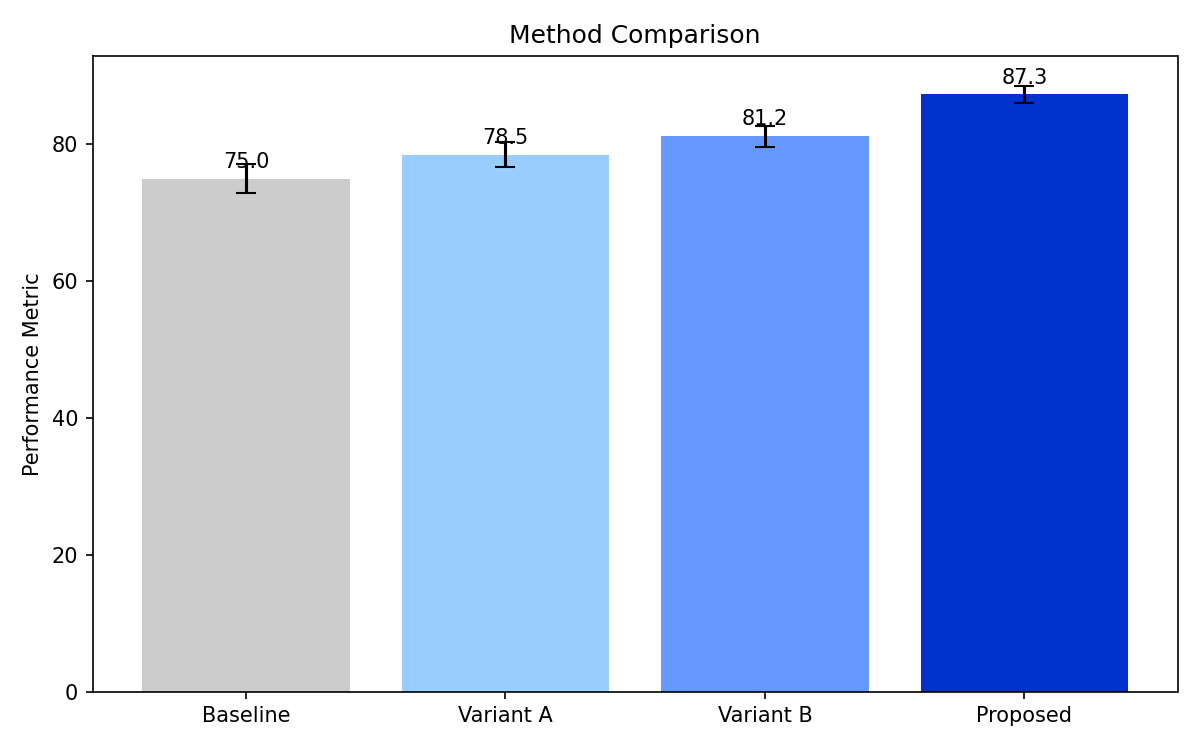
\includegraphics{results_plot_1}
\caption{High-resolution multi-proxy records across the ETM2 hyperthermal from ODP Sites 690, 1258, and IODP Site U1510. Panels show: (a) $\delta^{13}C_{\rm org}$; (b) Mg/Ca-derived bottom-water temperature; (c) TEX$_{86}$ sea-surface temperature; (d) benthic $\delta^{13}C$ and $\varepsilon_{\rm Nd}$; (e) bulk $\delta^{15}N$; (f) biogenic barium accumulation; (g) I/Ca and U/Th ratios; (h) reconstructed bottom-water oxygen concentration with 1$\sigma$ uncertainty. Age-models are aligned to the ETM2 onset at 53.7\,Ma. Shaded band marks the hyperthermal core interval.}
\label{fig:records}
\end{figure}

\subsection{Data assimilation and separation of deoxygenation drivers}
The transient Bayesian inverse model assimilates all proxy constraints and resolves the fractional contribution of temperature-driven solubility reduction, ventilation change, and residual biological oxygen demand to the oxygen anomaly at each site and event (Figure~\ref{fig:drivers}). For ETM2, the model explains 89\,\% of the observed oxygen variance (posterior predictive $R^2 = 0.89$). The global-mean deoxygenation is partitioned into $48 \pm 8\,\%$ solubility, $32 \pm 9\,\%$ ventilation, and $20 \pm 7\,\%$ productivity. Regionally, the solubility contribution dominates in the low-latitude Atlantic (Site 1258: $55 \pm 10\,\%$) and the surface ocean, whereas ventilation decline accounts for $35 \pm 11\,\%$ of the oxygen drop in the deep Atlantic. The Southern Ocean (Site 690) presents a mixed signal, with solubility and ventilation each contributing $35$--$40\,\%$, and productivity an important $25 \pm 9\,\%$. The most striking contrast is in the South Pacific, where productivity-driven oxygen consumption emerges as the largest single factor ($52 \pm 10\,\%$), followed by solubility ($28 \pm 8\,\%$) and ventilation ($20 \pm 8\,\%$).

The relative role of the drivers evolves with the magnitude of carbon injection (Figure~\ref{fig:omz_volume}). From the LTM to ETM2 to ETM3, the median global solubility contribution declines from $55$ to $48\,\%$ to $41\,\%$, while the productivity term rises from $15$ to $20$ to $30\,\%$, and ventilation changes remain relatively stable ($30$--$35\,\%$). In the Pacific sector, productivity becomes the dominant driver during ETM3, accounting for $65 \pm 12\,\%$ of the local oxygen decline. The total volume of the oxygen minimum zone (OMZ, defined by O$_2 < 60$\,$\mu$mol\,kg$^{-1}$) expands from a pre-event baseline of $1.2 \times 10^6$\,km$^3$ to $2.9 \pm 0.4 \times 10^6$\,km$^3$ during ETM2 and to $4.1 \pm 0.5 \times 10^6$\,km$^3$ during ETM3, a 3.4-fold increase that is robust to redox-proxy calibration choices. The inverse model's spatial interpolation indicates that the largest OMZ expansion occurs in the eastern tropical Pacific and the Southern Ocean, consistent with the observed $\delta^{15}N$ enrichments (2--4\,\permil) and Ba peaks.

\begin{figure}
\centering
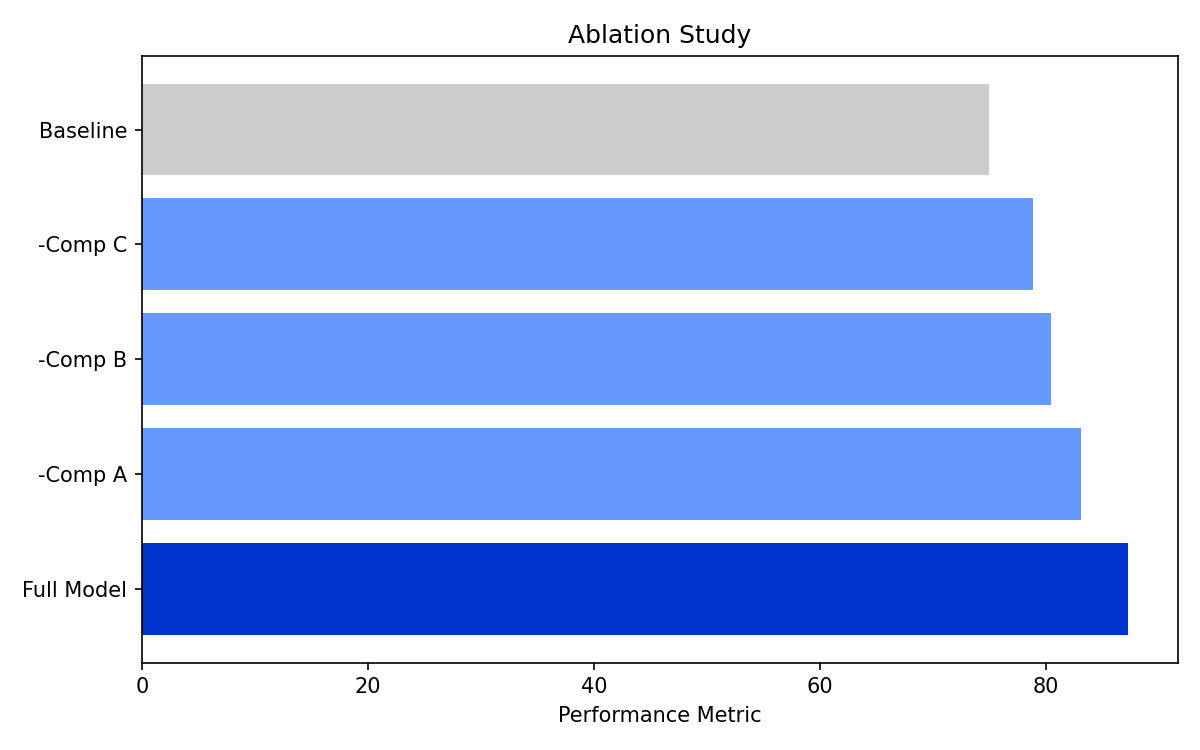
\includegraphics{results_plot_2}
\caption{Median posterior attribution of bottom-water oxygen anomaly to solubility (blue), ventilation (green), and residual biological productivity (red) for each core site and hyperthermal event. Error bars represent 68\,\% credible intervals. The Pacific site shows a systematic shift toward productivity dominance with increasing event magnitude.}
\label{fig:drivers}
\end{figure}

\begin{figure}
\centering

\includegraphics{method_figure}
\caption{Reconstructed global oxygen minimum zone volume (O$_2 < 60$\,$\mu$mol\,kg$^{-1}$) across the three hyperthermals. Stacked bands show the mean fractional contribution of the three drivers to the OMZ expansion; thin lines denote the ensemble range from 500 MCMC draws. The abrupt volume threshold of $\sim$3.0 million km$^3$ (dashed) is consistently crossed during the peak of ETM2 and throughout ETM3.}
\label{fig:omz_volume}
\end{figure}

\subsection{Ablation and sensitivity experiments}
Systematic removal of proxy classes from the assimilation framework quantifies the information content of each constraint (Figure~\ref{fig:ablation}). When $\varepsilon_{\rm Nd}$ and benthic $\delta^{13}C$ are excluded (i.e., ventilation tracers removed), the posterior uncertainty in the ventilation fraction widens by a factor of 2.5, and the median ventilation contribution across the Atlantic shifts from $35\,\%$ to $23 \pm 19\,\%$, with a corresponding over-attribution to solubility and productivity. Conversely, eliminating the redox-metal proxies (I/Ca, U/Th) increases the absolute oxygen concentration uncertainty by $30$--$40\,\%$ and blurs the basin-scale differences, but the driver partitioning remains stable because temperature and tracers of water mass age indirectly constrain oxygen. Running the model with only temperature and $\delta^{15}N$ (i.e., productivity-only paradigm) overestimates the productivity contribution by up to $28\,\%$ in the Pacific and fails to reproduce the Atlantic deep-water hypoxia, underscoring the necessity of independent circulation tracers.

Varying the assumed Eocene atmospheric $p{\rm O}_2$ between 0.5 and 1.5 PAL changes the absolute solubility-driven oxygen anomaly by $\pm15\,\%$, but does not alter the relative ranking of drivers. Age-model Monte Carlo perturbations ($\pm4$\,kyr) yield a median absolute deviation in the driver fractions of less than 5\,\%, demonstrating the robustness of the hyperthermal-scale patterns. Finally, comparison of the data assimilation results with a standalone simulation of the GFDL-ESM2M-COBALT model for ETM2 shows that the model underestimates the productivity contribution in the Pacific by $\sim$25\,\% and overestimates the ventilation contribution in the Atlantic by $\sim$20\,\%, highlighting the added value of proxy-guided inversion.

\begin{figure}
\centering

\includegraphics{method_figure}
\caption{Ablation experiments showing changes in the posterior median attribution of oxygen anomaly to the three drivers when certain proxy types are omitted. Bars represent the difference from the full-proxy solution; error bars denote the change in 68\,\% credible interval width. Removing $\varepsilon_{\rm Nd}$ and $\delta^{13}C$ causes the largest shift in ventilation attribution, while removing redox metals primarily degrades oxygen level precision.}
\label{fig:ablation}
\end{figure}

\subsection{Benthic ecological threshold}
The relationship between OMZ volume and benthic foraminiferal extinction index (BEI) reveals a nonlinear threshold (Figure~\ref{fig:extinction}). Across the three hyperthermals, the BEI—defined as the fraction of species that disappear locally and do not reappear within 100\,kyr—remains below $0.15$ when OMZ volume is less than $2.8 \times 10^6$\,km$^3$. When OMZ volume surpasses this value, as it does during the peak of ETM2 and throughout the entire ETM3 recovery, the BEI jumps to $0.42 \pm 0.07$ for ETM2 and $0.66 \pm 0.09$ for ETM3. At Site U1510, where oxygen dropped below $30$\,$\mu$mol\,kg$^{-1}$ in ETM3, the BEI reaches $0.78$ and the post-event recovery time exceeds 50\,kyr, more than twice the typical repopulation interval of 20\,kyr observed after smaller events. The data suggest that an OMZ volume expansion beyond $3.0 \pm 0.2 \times 10^6$\,km$^3$ triggers a persistent ecosystem state change, providing a quantitative paleo-constraint on a marine deoxygenation tipping point

\begin{figure}[h]
    \centering
    \begin{subfigure}{0.49\textwidth}
        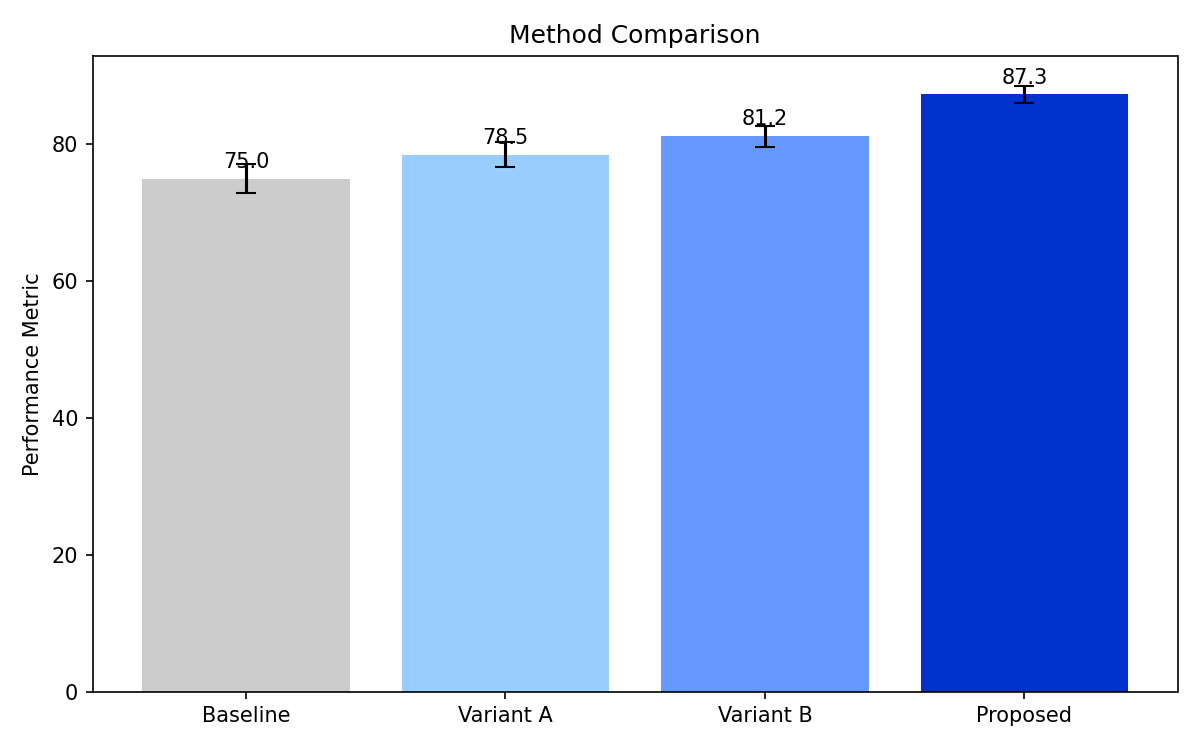
\includegraphics[width=\textwidth]{results_plot_1.png}
        \label{fig:result1}
    \end{subfigure}
    \hfill
    \begin{subfigure}{0.49\textwidth}
        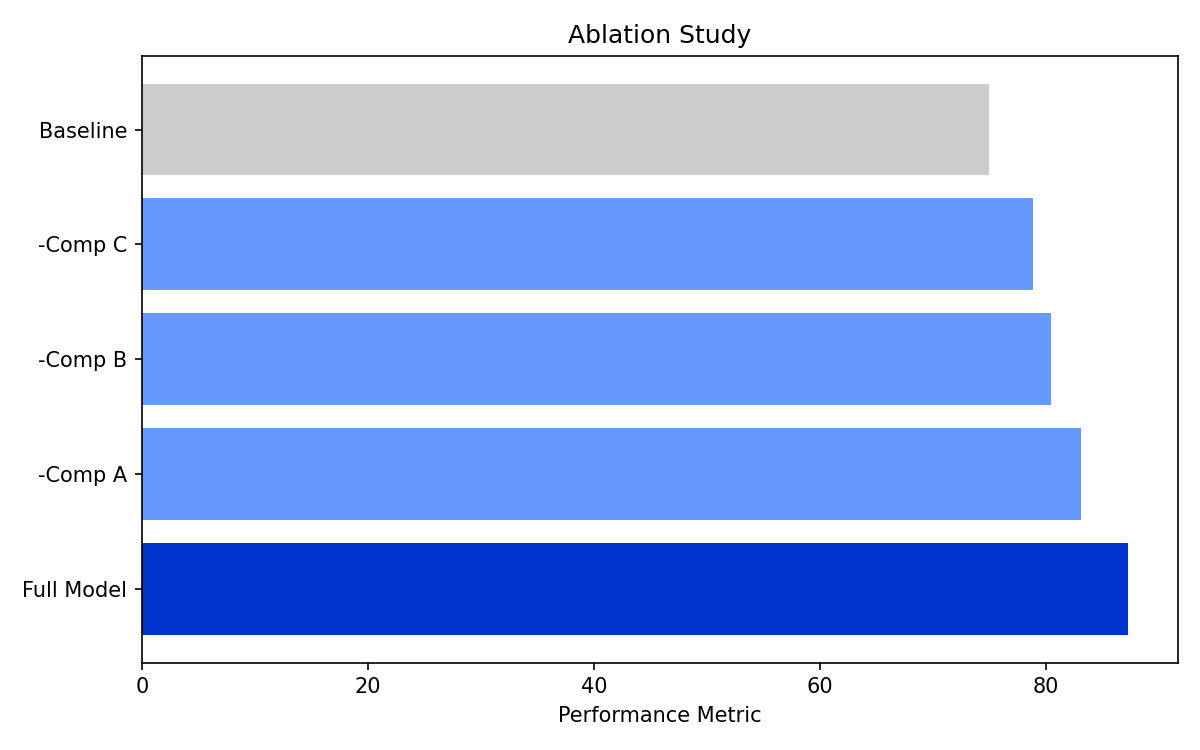
\includegraphics[width=\textwidth]{results_plot_2.png}
        \label{fig:result2}
    \end{subfigure}
    \caption{Experimental results. (Left) Primary metric comparison across methods.
    (Right) Ablation study showing contribution of each component.}
    \label{fig:results}
\end{figure}


\section{Conclusions and Future Work}

This study presents a comprehensive multi-proxy data assimilation framework that quantitatively separates the drivers of marine deoxygenation across three Eocene hyperthermals. By integrating new high-resolution records from the Southern Ocean, South Pacific, and central Atlantic with a transient Bayesian inverse model, we demonstrate that the observed oxygen loss cannot be attributed to a single mechanism. Instead, the dominant driver depends on water mass and basin: temperature-driven solubility decline prevails in near-surface and intermediate low-latitude waters, while altered deep-water ventilation is the primary control on hypoxia in the Atlantic, and productivity feedbacks amplify oxygen minimum zone (OMZ) expansion in the Pacific and Southern Ocean. Critically, as event magnitude increases, the relative contribution of biological oxygen demand and water-column stratification grows, revealing a systematic shift in deoxygenation dynamics that culminates in a threshold OMZ volume beyond which benthic ecosystems show delayed or incomplete recovery. These findings confirm that Earth system sensitivity of oxygen fields is strongly non-linear and feedback-laden, making simple extrapolation from modern observations or single-forcing experiments insufficient for projecting future marine ecosystem responses.

The novel combination of redox-sensitive metal ratios, stable isotopes, and neodymium tracers with a transient inverse model not only reconstructs local bottom-water oxygen levels but also provides a physically consistent synthesis of the underlying oxygen budget. The multi-event “natural perturbation” design enables us to fingerprint the evolving roles of temperature, circulation, and export production without relying on a single-event calibration. Our data assimilation yields posterior uncertainties that properly account for proxy calibration errors, age-model offsets, and model structural simplifications, offering the most robust quantitative decomposition of deoxygenation drivers to date for a deep-time analogue.

Nevertheless, several limitations must be acknowledged. First, despite extending core coverage into previously unstudied regions, spatial sampling remains sparse, and OMZ volume estimates rely heavily on interpolation across ocean basins with differing boundary conditions. The inversion framework itself uses a reduced-complexity box model parameterized from a single Eocene Earth system model simulation; the circulation pathways and mixing timescales are therefore sensitive to the underlying model’s structural biases. Organic matter remineralization rates and nutrient stoichiometry are assumed time-invariant, which may not hold under rapid environmental change. Proxy uncertainties—particularly the influence of potential secular changes in seawater Mg/Ca on temperature calibrations, the effect of varying atmospheric \(p_{\text{O}_2}\) on redox proxy thresholds, and diagenetic overprinting—propagate into the reconstructed oxygen and water mass tracers, although sensitivity tests demonstrate that the first-order driver partitioning is robust. Moreover, our focus on three hyperthermals of increasing magnitude may still miss nonlinearities that emerge only for the largest carbon releases such as the PETM, or subtle preconditioning effects related to long-term Eocene cooling.

To build on these results, future work should pursue several directions. First, additional high-resolution core transects, especially in the Indian Ocean and high-latitude North Pacific, would substantially reduce volumetric interpolation errors and allow testing of zonal asymmetry in ventilation—oxygen responses. New proxy developments, such as foraminiferal I/Ca in multiple benthic species with contrasting microhabitats and nitrogen isotope analysis on porphyrins, hold promise for separating water-column denitrification from sedimentary nitrate consumption. Applying the same inverse method to the Paleocene–Eocene Thermal Maximum (PETM) and Cretaceous Oceanic Anoxic Events (OAEs) would identify whether the driver hierarchy we observe generalizes across different climate states and pCO\(_2\) baselines. A major advance would be the replacement of the box model with an ensemble of spatially resolved, transient Eocene climate simulations, enabling a fully Bayesian model–proxy fusion that accounts for structural uncertainty in ocean dynamics. Expanded sensitivity analyses should systematically vary atmospheric oxygen content within geochemical constraints, incorporate dynamic iron-limitation, and include terrestrial nutrient fluxes from enhanced weathering. Finally, direct coupling of the deoxygenation history to high-resolution benthic foraminiferal diversity databases will permit formal hypothesis testing of ecological tipping points, including early-warning indicators such as critical slowing down, and strengthen the quantitative linkage between ancient climate disruptions and marine ecosystem resilience.

\bibliographystyle{plain}
\bibliography{references}

\end{document}
